\documentclass{article}

\usepackage[main=english,vietnamese]{babel}
\usepackage[T1]{fontenc}
\usepackage[utf8]{inputenc}
\usepackage[sexy]{evan}
\usepackage{matchsticks}
\usepackage{wrapfig}
\usepackage{listings}

\newtheorem{hint}{Hint}

\title{Solving Forty Two Problems by the Induction Principle - Part III}
\author{Nghia Doan}
\date{\today}

\begin{document}

\maketitle

\begin{problem}[Problem Eleven]
    Let $A_1A_2 \ldots A_n$ be a convex polygon inscribed in a circle such that among its vertices, there are no two which form a diameter.
    Prove that if among the triangles $A_p A_q A_r$ as distinct $p,q,r$ range over $1,2,\ldots,n,$ there is at least one acute triangle, then there are at least $n-2$ such acute triangle.
\end{problem}

\begin{soln}
    Let's prove it by induction based on $n$. The base case $n=3$ is simple to verify.
    Let $n \ge 4.$ Let $\triangle A_p A_q A_r$ be an acute triangle and let's remove an vertex $A_k$ distinct from $A_p, A_q, A_r$ ($1 \le k \le n$, $k \not \in \{p, q, r\}$)
    The induction hypothesis now should be true for the newly obtained $(n-1)-$gon,
    there are $n-3$ acute triangles with vertexes among $\{A_i, i=1,2,\ldots, n\} \setminus \{A_k\}$. 

    Now, WLOG, let's assume that $A_k \in \arc{A_pA_q}.$ Consider $\angle A_k A_p A_r$ and $\angle A_k A_q A_r.$
    They can not be equal, which then implies that $A_r A_k$ is a diameter. Thus one is strictly less than the other.
    Let assume that $\angle A_k A_p A_r < \angle A_k A_q A_r.$ then $\angle A_k A_p A_r < 90\dg.$
    
    \begin{center}
        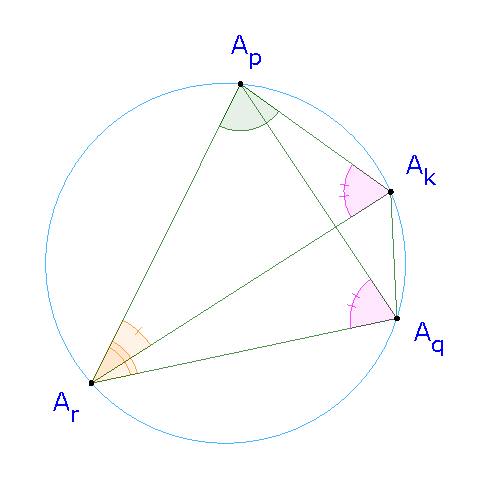
\includegraphics[width=6.5cm]{./svg/pdf/23-24-s5-o-p9.pdf}
    \end{center}

    In this $\triangle A_k A_p A_r,$ from above $\angle A_k A_p A_r < 90\dg;$ 
    $\angle A_p A_k A_r = \angle A_p A_q A_r < 90\dg$ (because $\triangle A_p A_q A_r$ is acute);
    and $\angle A_p A_r A_k < \angle A_p A_r A_q < 90\dg.$ Therefore $\triangle A_k A_p A_r$ is acute.

    This $\triangle A_k A_p A_r$ acute triangle is distinct from the other $n-3$ acute triangles in the $(n-1)-$gon,
    and together with them make $n-2$ acute triangles in the $n-$gon.

    The hypothesis is now proven for $n$ and thus should be true for all $n\ge 3.$
\end{soln}

\begin{problem}[Problem Twelf]
    There are 56 candies on the table, Players play by turns (one after another).
    In each turn it is allowed to take either one, three, or five candies.
    The winner is the person who takes the last set of candies.
    Given the perfect play on both sides, who will win?

    Three players play the following game. There are 54 candies on the table. Players play by turns (one after the other).
    In each turn it is allow to take either one, three, or five candies such that the same number of candies cannot be taken in two consecutive turns.
    The winner is the person who takes the last set of candies.
    Given the perfect play of all players, who will win?
\end{problem}

\begin{soln}
    For the first question, we prove that if the number of candies is in $6n-4$ format then the second player wins.
    It is easy to see that the base case is true.
    For $6(n+1)-4$ candies ($n\ge 1$), the second player always take $6-k$ candies if the first player takes $k$ candies in the first round,
    thus leading the game back to a \textit{known winning position.}

    For the second game, we prove by induction based on $9n,$ the number of candies.
    For $n=1,$ the first two players can take altogether 4, 6, or 8, candies which means that the third player will always win.
    Let that be the assumption for $9n.$ For $9(n+1)$ candies, the third player can always finish the first round such that there remains $9n$ candies,
    thus leading the game back to a \textit{known winning position.}
\end{soln}

\begin{problem}[Problem Thirteen]
    Prove that every positive integer $n \ge 2$ is expressible as a product of primes in exactly one way.
    In particular, if 
    \[
        p_1 p_2 \cdots p_k = q_1 q_2 \cdot q_{\ell},\ \text{where } p_1, p_2, \ldots p_k, q_1, q_2, \ldots q_l \text{\ are primes,}
    \]
    then $k = l$ and $q_1, q_2, \ldots q_l$ are $p_1, p_2, \ldots p_k$ in some order.
\end{problem}

\begin{soln}
    We prove the statement in two parts.
    \begin{claim*}
        Every positive integer $n \ge 2$ is expressible as a product of primes.
    \end{claim*}
    \begin{subproof}
        Assume the contrary, then by the Extremal principle, there exists a minimal $n$ that cannot be written as product of primes.
        If $n$ is a prime, then it is a product of one prime, thus $n$ is not a prime. Then there exist $1 < a, b < n$ integers such that
        $n=a\cdot b.$ By the Extremal principle, $a$ and $b$ must be product of primes, thus $n$ is.
        This is a contradiction, thus $n$ is expressible as a product of primes.
    \end{subproof}

    \begin{claim*}
        There is a single way to express $n$ as a product of primes.
    \end{claim*}
    \begin{subproof}
        We prove by induction on $k+\ell,$ in other words
        \[
            n = p_1 p_2 \cdots p_k = q_1 q_2 \cdot q_{\ell},\ \text{where } p_1, p_2, \ldots p_k, q_1, q_2, \ldots q_{\ell} \text{\ are primes,}
        \]
        then $k = \ell$ and $q_1, q_2, \ldots q_{\ell}$ are $p_1, p_2, \ldots p_k$ in some order.

        It is easy to see that if $k+\ell=2,$ then $k=\ell=1,$ otherwise we have 1 as a product of two primes, which is impossible.

        Now consider the case $l+k,$
        \[
            p_1 p_2 \cdots p_k = q_1 q_2 \cdot q_{\ell} \Rightarrow p_1 \mid q_1 q_2 \cdot q_{\ell} \Rightarrow \exists i \in \{1,\ldots,\ell\} p_1 \mid q_i 
            \Rightarrow p_1 = q_i \Rightarrow  p_2 \cdots p_k = q_1 \cdots q_{i-1} q_{i+1} \cdots q_{\ell}
        \]

        By the induction hypothesis for $k+\ell-2,$ $k=1=\ell-1,$ $q_1, \ldots, q_{i-1}, q_{i+1} \ldots q_{\ell}$ are $p_2, \ldots p_k.$
        Thus $k = \ell,$ and $q_1, q_2, \ldots q_{\ell}$ are $p_1, p_2, \ldots p_k$ in some order.

        Therefore the statement stands.
    \end{subproof}
\end{soln}

\begin{problem}[Problem Fourteen]
    Let $n$ be a positive integer. Does $n^2$ have more positive divisors of the form $4k+1$ or of the form $4k-1$?
\end{problem}

\begin{soln}
    Let $M(n)$ be the number of positive divisors of $n^2$ in the form $4k-1$, $P(n)$ be the number of positive divisors of $n^2$ in the form $4k+1$. 

    It is easy to see that $M(2^k) = 0 < 1 = P(2^k).$

    We prove by strong induction based on the number of prime powers in prime factorization of $n,$
    \begin{claim*}
        $M(n) < P(n).$
    \end{claim*}
    \begin{subproof}
        Let $p$ be a prime such that $p \not |\ n,\ p \equiv 1 \Mod{4}.$
        Then every divisor of $(p^{\alpha}n)^2 = p^{2\alpha}n^2$ of the form $4k-1$ is a power of $p$ times a divisor of $n^2$ of the form $4k-1$. 
        
        Similarly every divisor of $(p^{\alpha}n)^2 = p^{2\alpha}n^2$ of the form $4k+1$ is a power of $p$ times a divisor of $n^2$ of the form $4k+1$.
        Hence 
        \[
            \begin{aligned}
                &M(p^{\alpha}n)=(2\alpha_1)M(n),\ P(p^{\alpha}n)=(2\alpha_1)P(n)\\
                &M(n) < P(n) \Rightarrow M(p^{\alpha}n) < P(p^{\alpha}n) \quad (*)
            \end{aligned}
        \]

        Now, consider $p$ be a prime such that $p \not |\ n,\ p \equiv -1 \Mod{4}.$
        Then every divisor of $(p^{\alpha}n)^2 = p^{2\alpha}n^2$ of the form $4k-1$ is either $p^{2r}$ times a divisor of $n^2$ of the form $4k-1$
        ($0 \le r \le \alpha$) or $p^{2r-1}$ times a divisor of $n^2$ of the form $4k+1$ ($1 \le r \le \alpha$).
        
        Similarly every divisor of $(p^{\alpha}n)^2 = p^{2\alpha}n^2$ of the form $4k+1$ is either $p^{2r}$ times a divisor of $n^2$ of the form $4k+1$
        ($0 \le r \le \alpha$) or $p^{2r-1}$ times a divisor of $n^2$ of the form $4k-1$ ($1 \le r \le \alpha$).
        Hence 
        \[
            \begin{aligned}
                &M(p^{\alpha}n)=(\alpha_1+1)M(n) + \alpha P(n),\ P(p^{\alpha}n)=(\alpha_1+1)P(n) + \alpha M(n)\\
                &M(n) < P(n) \Rightarrow M(p^{\alpha}n) < P(p^{\alpha}n) \quad (**)
            \end{aligned}
        \]

        (*) and (**) imply that the hypothesis stands for $p^{\alpha}n.$
    \end{subproof}
\end{soln}

\begin{problem}[Problem Fifteen]
    Prove that for all $n \in \ZZ^+.$

    (a) $17 \mid 2^{5n+3} + 5^n\cdot 3^{n+2}.$

    (b) $p \mid n^p - n,$ for any $p$ prime.
\end{problem}

\begin{soln}
    Let $P(n):\ 17 \mid 2^{5n+3} + 5^n\cdot 3^{n+2}.$ Then $P(0)$ is true because $17 \mid 2^3 + 5^0 \cdot 3^2 = 17.$
    Assume $P(k)$ is true, for all $k \le n,$ then
    \[
        \begin{aligned}
            &2^{5(n+1)+3} + 5^{n+1}\cdot 3^{(n+1)+2} = 2^{5n+8} + 5^{n+1}\cdot 3^{n+3}\\
            &=(2^{5n+3} \cdot 34 - 2^{5n+3} \cdot 2) + (5^n\cdot 3^{n+2} \cdot 17 - 5^n \cdot 3^{n+2} \cdot 2)\\
            &= 2^{5n+3} \cdot 17 + 17(2^{5n+3} + 5^n\cdot 3^{n+2}) - 2(2^{5n+3} + 5^n \cdot 3^{n+2}) \quad (*)
        \end{aligned}
    \]
    
    The expression in (*) is a multiple of $17,$ thus $P(n+1)$ is true.
    Therefore $P(n)$ is true for all $n.$

    For the second question, let analyze the inductive step. Note that
    \[
        (n+1)^p - (n+1) = \left(n^p + \binom{p}{1} n^{p-1} + \cdots + \binom{p}{p-1} n + 1 \right) - (n+1)
    \]

    Since $\binom{p}{i} = p \cdot \frac{(p-1)!}{i!(p-i)},$ thus it is a multiple of $p,$
    therefore the inductive step is obvious base on $p \mid n^p - n.$
\end{soln}

\end{document}